%
% File acl2015.tex
%
% Contact: car@ir.hit.edu.cn, gdzhou@suda.edu.cn
%%
%% Based on the style files for ACL-2014, which were, in turn,
%% Based on the style files for ACL-2013, which were, in turn,
%% Based on the style files for ACL-2012, which were, in turn,
%% based on the style files for ACL-2011, which were, in turn,
%% based on the style files for ACL-2010, which were, in turn,
%% based on the style files for ACL-IJCNLP-2009, which were, in turn,
%% based on the style files for EACL-2009 and IJCNLP-2008...

%% Based on the style files for EACL 2006 by
%%e.agirre@ehu.es or Sergi.Balari@uab.es
%% and that of ACL 08 by Joakim Nivre and Noah Smith

\documentclass[11pt]{article}
\usepackage{acl2015}
\usepackage{times}
\usepackage{hyperref}
\usepackage{latexsym}
\usepackage{color}
\usepackage{amsmath}
\usepackage{epsfig}
\usepackage{graphicx}
\newcommand{\figref}[1]{Figure \ref{#1}}
\newcommand{\tabref}[1]{Table \ref{#1}}
\usepackage{epstopdf}
\usepackage{booktabs}
\usepackage{diagbox}
\usepackage{array}
%\usepackage{float}
\usepackage{stfloats}
\usepackage{multicol}
\usepackage{threeparttable}
\usepackage[multiple]{footmisc}

%\usepackage[skip=2pt,font=scriptsize]{caption}
\newcolumntype{I}{!{\vrule width 1pt}}
\newlength\savedwidth
\newcommand\whline{\noalign{\global\savedwidth\arrayrulewidth
                            \global\arrayrulewidth 1pt}%
                   \hline
                   \noalign{\global\arrayrulewidth\savedwidth}}
\newlength{\Oldarrayrulewidth}
\newcommand{\Cline}[2]{%
  \noalign{\global\setlength{\Oldarrayrulewidth}{\arrayrulewidth}}%
  \noalign{\global\setlength{\arrayrulewidth}{#1}}\cline{#2}%
  \noalign{\global\setlength{\arrayrulewidth}{\Oldarrayrulewidth}}}

\newcommand{\KZ}[1]{\textcolor{blue}{Kenny: #1}}
\newcommand{\BF}[1]{\textcolor{red}{Bean: #1}}
\newcommand{\TJ}[1]{\textcolor{red}{Jia: #1}}
\newcommand{\YZ}[1]{\textcolor{red}{Yizhong: #1}}
\newcommand{\cut}[1]{}


% You can expand the titlebox if you need extra space
% to show all the authors. Please do not make the titlebox
% smaller than 5cm (the original size); we will check this
% in the camera-ready version and ask you to change it back.


\title{BeanParser: A Sequence-based Dependency Parser}

\author{Wenjing Fang \and Yizhong Wang \and Jia Tan \and Kenny Q. Zhu  \\
  Shanghai Jiao Tong University \\
  {\tt littlebeanfang@sjtu.edu.cn}, {\tt kzhu@cs.sjtu.edu.cn} \\
  }
%\date{}

\begin{document}
\maketitle
\begin{abstract}
%Existing data-driven dependency parsers mainly fall into two classes:
%graph-based and transition-based. However, both methods draw some distinctions
%from the way that we human beings perform the parsing task.
This paper demonstrates a novel dependency parsing framework that
imitates how a human parses sentences in an intuitive way.
At every step of the parse, it determines which word is the easiest to
process among all the remaining words, identifies its head word and then
folds it under the head word.
This greedy framework achieves competitive accuracy on WSJ evaluation set
and shows additional advantage on the non-projective corpus.
%\BF{multi-lingual}
 % \BF{redo experiment,not the accurate number}
Further, this work is flexible enough to be augmented with other
parsing techniques.
\end{abstract}
\section{Introduction}

Protein$-$protein interactions (PPIs) are of central importance for the majority of biological functions, such as signal transduction, metabolic pathways, molecular dynamics, and protein networks\cite{Hoffmann.Krallinger.ea:2005}, for they serve as the most fundamental building blocks of the entire interacademic systems of any organisms. Collecting data on pairwise interaction relationships is essential for multiple purpose, including identification of modules with certain functionality\cite{Spirin.Mirny.03}, mapping diseases to dominated genes\cite{Ideker.Sharan.08}, and after all, understanding wholistic metabolic/genetic networks from a system biology perspective.

A lot of databases have been built to store protein and genetic interactions from major model organism species and are available in various standardized formats, such as MINT\cite{Zanzoni.Montecchi-Palazzi.ea:2002}, BIND\cite{Bader.ea:2003}, BIOGRID\cite{DBLP:journals/nar/StarkBRBBT06}, etc. Among those mainstream databases, the data largely rely on voluntary reports by scientists or researchers, besides, comprehensive curation efforts become indispensable for the sake of accuracy. However, the amount of biology-related literatures with respect to protein interactions grows explosively and thus make it either impossible or impractical to manually detect PPI information anymore.

Considering huge amount of PPI information with great wealth hidden in published papers, in recent years, numerous mining techniques have been proposed that aim to extract PPI information automatically from free text, especially machine learning, information retrieval, and natural language processing\cite{DBLP:journals/bib/WinnenburgWPDS08}.These approaches can be roughly categorized into three classes: co$-$occurrence, rule$-$based, and machine learning. 

Co$-$occurrence is the approach with most simplicity and naivete. Just as its name implies, this method intends to find out pairs of proteins that co-occur in the same context. The scope of "same context" ranges from phrase, sentence, paragraph to whole abstract, even document. The underlying assumption is that whenever two proteins are mentioned together by authors, chances are high that there is some kind of relationship between them. However, however, in-context closeness even semantic relation does not necessarily represent actual biological interaction. As a consequence, a large fraction of candidate pairs are mismatched inevitably, causing a high recall but low precision.

The second approach is rule-based extraction, in other words, pattern matching. There are many types of rules, most of them concern natural language processing (NLP). One way is to specify hand-crafted regular expressions before hand, which mostly lean on language usage preference. Besides, by using full or partial (shallow) parsing strategies, more information would be acquired, such as part-of-speech taggers, local dependencies between syntactic components, context-free grammar\cite{DBLP:journals/bioinformatics/TemkinG03}, and full sentence structure. Compared to co$-$occurrence, rule-based approach enjoy better precision but much lower recall. In addition, since the rules are usually derived from training data, that is to say, the improper choice of training data would be significantly lethal, therefore quality of extraction is invariably instable and may not applicable to other data.

The third and most commonly used approach use machine learning techniques, in this case, the task to extract protein$-$protein interactions turns out to be a binary classification problem. Each protein pairs are represented along with a set of features, which is associated with their context, then a well$-$defined classifier gives the answer whether the candidate protein pairs is classified to be qualified PPI. (TO BE FURTHER FILLED!!!)

In this paper, we introduce a general bootstrapping framework for Protein$-$protein interaction extraction from natural text.Our method differs from most of the previous works in three aspects:

(1)The extraction process is driven by only tiny fraction of training data, which are regarded as seed data. In each round, it would derive reliable patterns automatically from seed data, then extract more positive PPI pairs consequently, what's more, the seed data would be augmented by the newly extracted results with high confidence.

(2)multiple graph kernel. 

(3)various evaluation.





\section{Framework}
%\BF{workflow figure to show the framework}
%\begin{multicols}{2}
%\begin{figure*}
%\centering
%\includegraphics[width=2\columnwidth]{sysoverviewgrapheps.eps}
%\caption{Framework wrokflow} \label{fig:workflow}
%\end{figure*}
%\end{multicols}
%\KZ{In the framework, say ``Output Parse'' instead of ``Output File.''}
The general architecture of the our parser is shown in \figref{fig:workflow}
and is divided into training phase and parsing phase.
%We take training treebank as input, which carries the
%essential information (we only use FORM and POSTAG) and
%gold dependency parses.

\begin{figure}[th]
\centering
\epsfig{file=sysoverviewgrapheps.eps, width=\columnwidth}
\caption{Sequence Based Parser Framework}
\label{fig:workflow}
\end{figure}

{\bf Training:} The preprocessing step generates oracle sequences
from the gold standard parse trees. Only the word forms and the POS tags 
in these parse trees are used. Here, we assume that a child node is
easier to process than its parent node and it is supposed to be attached
before its parent. \footnote{By this rule, multiple gold sequences
can be generated from one dependency tree. In this paper, when a parent node
has multiple children, we generate the sequence by a left-to-right order.}
%\KZ{Which one do we use or do we use all of them?}
%\footnote{
%For example, a bottom-up, breadth-first traversal of the gold parse tree or oracle transition
%process order from Malt Parser are both gold sequences.}
%and further discussion is deferred to Section 4.
%\TJ{maybe they will ask which one is the best; needs some explanations here}
We then train respectively a graph-based head mapper (a.k.a. decoder)
from the gold sequences and the gold parses, and a sequence predictor
from the gold sequences.

{\bf Parsing:} Given an input sentence, the sequence predictor
outputs a feasible decoding sequence, which is a permutation of
the words in the input. For each word in this sequence,
the head mapper returns its best head word according to a scoring function
while employing a cycle detection mechanism.
The process continues until all words in the sentence have found their
heads.
%(except manually introduce ROOT node in dependency parsing).
%For a sentence with $N$ words, the final result consists of ($N+1$) nodes
%and constructed $N$ arcs.
The procedure guarantees to produce a tree structure eventually.
\cut{
We implemented a simple version of this framework,
%and released the source code as well as the evaluation data\footnote{\urlstyle{same}\url{https://github.com/littlebeanfang/BeanParser}}.
%To reproduce the experiments refered in this paper, all our data and related commands are offered in the compressed file.
%\BF{add the data download source}
%\KZ{Besides the open-source system, create an online demo using default model
%and allow users to type in
%a sentence to have it parsed.}
and built an online demo\footnote{\urlstyle{same}\url{http://202.120.38.146/BeanParser}} to show parses of eight languages with the model
trained in our experiment.}

In the current implementation, we generate the decoding sequence by
{\em stackproj} algorithm~\cite{nivre2009non} in
malt parser and scorer-based greedy head mapper.
%\KZ{Consider rephrase this sentence.
%What does graph-based head mapper have to do with sequence?}
%The training and testing data are both in
%CoNLL format~\footnote{http://ilk.uvt.nl/conll/}.



\section{Head Mapper}
%	* high order feature: arc heat change, influence of 2 order feature, feature template
%	* learning: MIRA, converge of training
%	* pseudocode of mapper(avoid circle) framework
%\KZ{Rephrase the following. What do you mean by attach? Also try not to be too casual, e.g., think about...}
%\BF{Mcdonald's example graph of decoding: ROOT John saw a dog yesterday which was a Yorkshire Terrier.}
In this section, we first give an example to explain how head mapper actually works. Then we explain
the features and scorer embeded in the head mapper. Finally, we describe the method to train the scorer model.

%\KZ{Figure needs to be restored to original one as some letters are missing.}

\begin{figure*}[th]
\centering
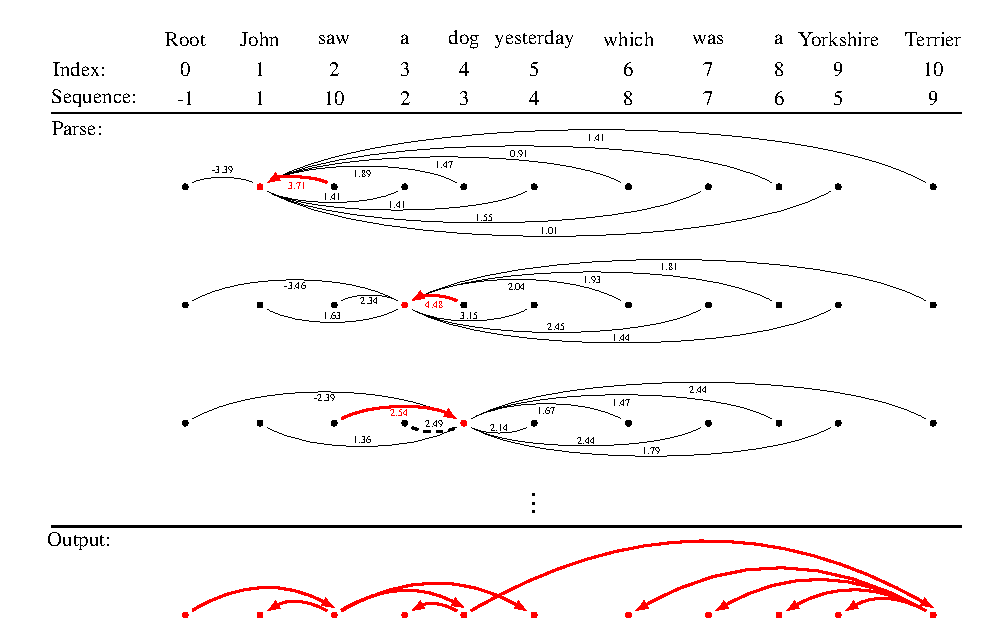
\epsfig{file=exampleparse_chg.eps, width=1.8\columnwidth}
\caption{Example Parse of head mapper}
%for the sentence ``\emph{John saw a dog yesterday which was a Yorkshire Terrier}". Red node is the child to be processed in every step; red arc is the final attachment from head to its dependent and dashed arc is left out to avoid circle in the parse tree.}
\label{fig:egparse}
\end{figure*}

\subsection{Parsing}
\figref{fig:egparse} shows the decoding process of the head mapper
for a non-projective example sentence previously used \cite{mcdonald2005non}.
%\KZ{You don't have to repeat the CoNNL format. It's not important.}
%Pseudocode shows how the head mapper works.
%Our decoder works just as the process in \figref{fig:egparse}.
%\BF{pseudocode of head mapper decoding and symbol explainations here}
A head mapper takes lexical information of a sentence and
a permutation sequence of words in that sentence as inputs.
The sequence of the sentence is:% from MaltParser:
$John_{1}\rightarrow a_{3}\rightarrow dog_{4}\rightarrow yesterday_{5}\rightarrow Yorkshire_{9}\rightarrow a_{8}\rightarrow was_{7}\rightarrow which_{6}\rightarrow Terrier_{10}\rightarrow saw_{2}$.
In step one, we look for the head of \textit{John} and
all the other words are potential candidate head. In order to measure
the probabilities of these candidate arcs, we introduce a scorer which
is the key idea of graph-based parsers. Judging from the scores
printed on every black arc in \figref{fig:egparse},
the red arc was eventually selected, i.e. $saw$ is taken to be the head
of $John$.  The process continues for the word \textit{a}, etc.

In practice, we maintain a disjoint set to ensure that
there are no cycles generated while parsing (e.g., in step 3 of
\figref{fig:egparse}),
so that the output is a dependency tree structure starting from
the ROOT node\footnote{A manually introduced node in dependency parsing task,
it is the root of a dependency tree}.
We also build a parse agenda to record the existing arcs which
provides the high order information for our scorer.
For a sentence with $N$ words, the final result consists of
($N+1$) nodes and constructed $N$ arcs.
%\KZ{You don't need to remind people over and over again this is a combination of
%MST and Malt. You just say what you did, if it's something that MST and Malt have
%done before, be very brief about this part, and give a citation. This paper
%is about your work, not about MST or Malt.}
%Both MaltParser and MSTParser treat projective and non-projective dependency tree discriminatively. MaltParser define an extra action SWAP to generate projectivization transformation of a non-projective dependency tree \cite{nivre2009non}.
%There is a drawback of MaltParser that it cannot generate non-projective output providing projective training set, because there are no SWAP action in oracle transitions. It is sensible to look into the relation between
%possible word pairs directly. But word order limits the word pairs considered in MaltParser. MSTParser employ Chu-Liu-Edmonds algorithm to decode non-projective cases \cite{mcdonald2005non}
%and Eisner algorithm to deal with projective trees\cite{mcdonald2005online}. Though Chu-Liu-Edmonds algorithm is a solution to unify projective and non-projective cases, it declines the accuracy while applying on projective trees. Our decoder also unifies these two situations and
%searches heads globally. It directly measures the relative closeness between every possible head and current processing word and generate non-projective tree naturally.
%Head mapper tries to map head for every word stepwise according to a given process sequence of words.
%\KZ{It makes sense to include an example here to illustrate the head-mapper.}

\subsection{Scorer and features}
%In order to simulate this process,
We introduce a linear arc scorer to measure the score of a directed arc.
The sum of all arc scores gives the final score of the whole parse tree.
%\BF{formula of arc score model}
%\[
%\text{Score}(\mathbf{y})=\displaystyle{\sum_{(i,j)\in\mathbf{y}}} \mathbf{w} \cdot \mathbf{f}(i,j)
%\]
%In this formula, $i,j$ are the indexes of an arc in parse tree $\mathbf{y}$. The inner product of arc feature vector $\mathbf{f}(i,j)$ and weight vector $\mathbf{w}$ represents score of an arc $(i,j)$. By summing up all the
%arc scores, we can get final score of the whole parse tree $\mathbf{y}$.
We currently use the same set of high-dimensional binary features as MSTParser,
%\BF{feature template table}
including second order features \cite{mcdonald2006online}.
%As the previous statement, feature scope in graph-based parser
%is limited by decoding algorithm and several works successfully
%adapt Eisner algorithm to include high order features .
Because of the deterministic decoding in our framework,
we can make use of existing arcs to guide later head mapping.
This kind of decoder gives us the flexibility of applying any
high order features explored by previous
works~\cite{carreras2007experiments,koo2010efficient,ma2012fourth}.

\subsection{Learning algorithm}
%\KZ{Again, you are making it sound like you only did some minor changes to MST.
%This is not the right style to write about your work. You can say we use a modified
%verion of MIRA~\cite{}, in which we did blah..}
%Based on different decoding and factoring methods, graph-based models employ different learning algorithms to induce the feature weights. Among them, variant perceptron algorithms are widely used \cite{kubler2009dependency}.
In this work, we adopt the iterative online training framework MIRA
(Margin Infused Relaxed Algorithm), which was used in the training process
of MSTParser. The updating constraint is defined as
\begin{align*}
&\text{min}\|\mathbf{w}^{(i+1)}-\mathbf{w}^{(i)}\|\\
&\text{s.t. } s(\boldsymbol{x}_t,\boldsymbol{y}_t)-s(\boldsymbol{x}_t,\boldsymbol{y}')\ge L(\boldsymbol{y}_t,\boldsymbol{y}')
%\\&\forall \boldsymbol{y}'\in \text{dt}(\boldsymbol{x}_t)
\end{align*}
where $\mathbf{w}^{(i)}$ are the feature weights for the $i$-th iteration,
$\mathbf{x}_t$ and $\mathbf{y}_t$ are sentence and its gold parse tree,
respectively. $\mathbf{y}'$ is the output of our parser with $\mathbf{w}^{(i)}$ and
score margin is given out by a loss function $L$.

%On each update, MIRA attempts to keep the norm of the change to the parameter vector as small as possible, subject to
%correctly classifying the instance under consideration with a margin at least as large as the loss of the incorrect classifications \cite{mcdonald2005online}.
%\BF{this is the original sentence in this paper}
%Similarly, we define the loss function as the number of incorrect arcs to apply MIRA to dependency parsing and it
%is represented as following formula: \BF{Is this formula necessary ?}
%\BF{MIRA formula}
%\KZ{Don't like the following sentence.}
%From this definition, the only change we should make is replacing the exact inference decoder with our deterministic
%decoder.
Every time, we update the feature weights based on one sentence. The
decoder gives a greedy parse according to current feature weights.
By scoring the gold dependency tree and the current parse,
along with the number of incorrect arcs in the current parse,
MIRA updates to eventually converge to an optimal scorer.
The learning algorithm typically terminates after a few iterations.
%(\figref{fig:itertest}).
%\BF{Converge graph of head mapper}
%\begin{figure}[htp]
%\centering
%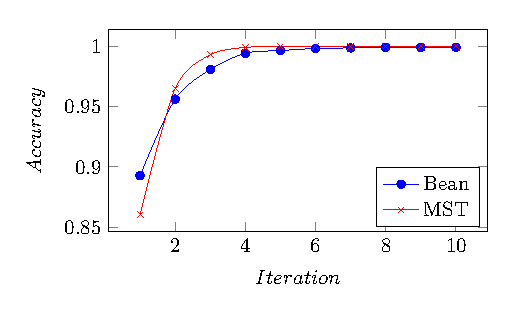
\epsfig{file=itertest.eps, width=\columnwidth}
%\caption{Accuracy curves on training set. \newline Test on first 100 sentence of WSJ senction 00.}
%\label{fig:itertest}
%\end{figure}


\section{Sequence Predictor}
%A sequence predictor either selects the word to process stepwise, or generates an complete word sequence.
We developed two types of sequence predictor. The first type is based on
offline training from ``gold'' parsing sequences, and produces a complete
parsing sequence given a sentence. The second type is unsupervised and is
integrated with the decoding process, i.e. it produces the next word to
process based on the current parsing configuration.
We divide the first type of predictor into two approaches, one by a learning
to rank algorithm, and second by an action classifier used in MaltParser.
Next we briefly discuss these three approaches.

%We state the rule of gold sequence in Section 2 and we can generate gold sequences with the gold dependency trees.
%Sequence predictor then learns from these gold sequences and tries to produce a sequence
%for new sentences.
%
%\subsection{Effects of Sequences}
%\KZ{Not sure what ``Sequence dependence'' means. Headings should be self-explanatory
%and clean. Consider rephrase the following paragraph. Very garbbled.}
%As we point out in section 2, getting a gold sequence from a gold dependency tree is not a one-to-one mapping.
%\BF{breadth-first traversal and malt convert sequences of example sentence}
%For example, there is a breadth-first traversal sequence of the sentence in \figref{fig:egparse},
%$which_{6}\rightarrow was_{7}\rightarrow a_{8}\rightarrow Yorkshire_{9}\rightarrow a_{3}\rightarrow Terrier_{10}\rightarrow John_{1}\rightarrow dog_{4}\rightarrow yesterday_{5}\rightarrow saw_{2}$
%, which is also a gold sequence along with the example sequence.

\subsection{Pairwise learning to rank}
\cut{In this approach, we attempted two ways to generate gold parsing sequences.
First is a bottom-up, breadth-first traversal of the gold parse tree. This
way we are essentially processing words which are lower down in the parse
tree first, which are often less important modifiers, before moving to words
which are more central to the syntactic structure of the sentence.
The second is to take the training data from a converting function of
MaltParser, which converts a gold parse tree into a sequence of actions.
We can infer the parsing sequence of words from the sequence of actions.}

%We human beings execute a few pairwise comparisons to decide the next
%word to be processed, which is similar to preference learning problem in learning to rank.
%Sequence predicting is also a ranking process. We select next word to process by comparing it with the other words in a pairwise way.
%Viewing the task of sequence predictor in this way,
%preference learning problem in learning to rank gives a solution to predict.
We can decompose a gold sequence into pairwise partial orders between
two words and train a binary classifer to determine the order of any two
words within a sentence. This is a popular approach in learning to rank.
However, combining pairwise orders into a complete sequence is an NP
problem~\cite{grotschel1984cutting}, we therefore use a greedy algorithm
from Cohen \cite{schapire1998learning} to produce such a sequence.

\subsection{Action classifier in MaltParser}
MaltParser employs a classifier to determine what parsing action (e.g.,
{\em shift}, {\em push}, etc.) to take at each step. The whole parsing
process defines a sequence of such actions. Although this sequence is
not exactly the word sequence used in our system, such a word sequence
can be inferred rather straightforwardly from the action sequence.
Another advantage of
the MaltParser is that it's extremely fast. Therefore, we can use MaltParser
to quickly parse through a given sentence, record the action sequence and
infer the parse sequence from it.

%
%Inspired by our left-to-right analysis of a sentence, we either find
%head for current word or skip this hard word and scan on. This is obviously a classification problem and
%MaltParser happen to hold the same view.\BF{cannot say so now} MaltParser add arc incrementally and provide us a potential sequence.
%In fact, we can understand the action classifier in a different way that it can reflect the relative
%priority between the top two words on processing stack. So, we translate the action as:
% LA - process the word on the top of stack;
% RA - process the second word in stack;
% SH - postpone the process of both the two words on top of stack.


%We can decompose the predicting process into two steps:
%getting pairwise rank of every two nodes and aggregating
%these partial results into a complete process sequence.
%
%We apply LIBLINEAR\footnote{\urlstyle{same}\url{http://www.csie.ntu.edu.tw/~cjlin/liblinear/}} to training a binary classifier to get the priority of every two words. The training data are pairwise orders extracted from the gold sequence.
%The classifier can then be used to predict the relative ordering for any two words with a confidence score.
%\BF{Jia fill the details: rankSVM, Cohen, citation of preference learning}

%  \item {\bf Malt} The oracle sequence generated by converting function in MaltParser.
%  \item {\bf Random} A random permutation sequence of words for a sentence.
%  \item {\bf Increase} The left-to-right sequence, which means we process the sentence with
%  the word index increasing.
%\end{itemize}
%
%In order to test how the sequence quality influence decoding and measure different types of sequences,
%we generate four types of sequence files to test on the head mapper.
%%The train set is transformed by StanfordParser on WSJ section 2-21 and test set on WSJ section 00-01.
%Types of sequences are list below:
%Among them, the Malt sequence outperforms other types of the sequences.
%In the following, we describe a few alternative approaches to predict the sequences.
%%        \item[1] The breadth-first traversal sequence of a sentence
%        \item[2] The oracle sequence generated by converting function in MaltParser.
%        \item[3] Predicting process sequence of MaltParser stackproj algorithm.
%        \item[4] The random permutation sequence of words in a sentence.
%        \item[5] The left to right sequence, word indexes are process sequences.
%{\bf Breadth-first} The breadth-first traversal sequence of a sentence.
%
%{\bf MaltConvert} The oracle sequence generated by converting function in MaltParser.
%
%{\bf MaltPredict} Predicting process sequence of MaltParser stackproj algorithm.
%
%{\bf Random} The random permutation sequence of words in a sentence.
%
%{\bf Increase} The left to right sequence, word indexes are process sequences.
%{\small
%~\\
%
%$\bullet$ Oracle {\bf converting} sequences of MaltParser.
%
%$\bullet$ {\bf Breadth-first} traversal of a gold parse tree.
%
%$\bullet$ {\bf Predicting} process sequence of MaltParser.
%
%$\bullet$ A {\bf random} words permutation of the sentence.
%
%$\bullet$ A word sequence with {\bf increasing} index from left to right of the sentence.
%\begin{table*}[htbp]
%  \centering
%  \caption{Cross test of sequence type}
%  %\begin{threeparttable}
%    \begin{tabular}{Il|cccccIccI}
%    \whline
%    %\diagbox{Test}{Train}& Breadth-first\tnote{1} & MaltConvert\tnote{2} & MaltPredict\tnote{3} & Random\tnote{4} & Increase\tnote{5} & Average & StdDev \\
%    \diagbox{Test}{Train}& MaltConvert & Breadth-first & MaltPredict & Random & Increase & Average & StdDev \\
%    \hline
%    MaltConvert & 93.59\% & 67.32\%  & 93.29\% & 89.50\% & 83.91\% & 85.52\% & 0.109 \\
%    Breadth-first & 79.65\% & 92.36\% & 80.93\% & 86.46\% & 84.75\% & 84.83\% & 0.050 \\
%    MaltPredict & 89.30\% & 66.07\%  & 89.50\% & 87.14\% & 82.36\% & 82.87\% & 0.098 \\
%    Random & 55.41\% & 48.84\% & 56.49\% & 70.92\% & 62.77\% & 58.89\% & 0.083 \\
%    Increase & 48.89\% & 46.98\% & 48.83\% & 65.18\% & 63.36\% & 54.65\% & 0.088 \\[2pt]
%    \whline
%    \hline
%    %\midrule[3pt]
%    %     &       &       &       &       &       &     &  \\
%    Average & 73.37\% & 64.31\% & 73.81\% & 79.84\% & 75.43\%      &     & \\
%    StdDev & 0.201 & 0.183 & 0.200 & 0.110 & 0.113     &     & \\
%    \Cline{1.5pt}{1-8}
%    \end{tabular}%
%    %\begin{tablenotes}
%%        \footnotesize
%%        \item[1] The breadth-first traversal sequence of a sentence
%%        \item[2] The oracle sequence generated by converting function in MaltParser.
%%        \item[3] Predicting process sequence of MaltParser stackproj algorithm.
%%        \item[4] The random permutation sequence of words in a sentence.
%%        \item[5] The left to right sequence, word indexes are process sequences.
%%      \end{tablenotes}
%%\end{threeparttable}
%  \label{tab:crosstest}%
%\end{table*}%
%\subsection{Attempts}


\subsection{Feature score based predictor}
%{\bf Scorer-based  }
The intuition of sequence predictor is to rank words
according to the ease of head word attaching.
Words that are easy to handle can be processed earlier without high order features.
\cut{Words that are processed later are harder and may require high order
features. Such high order features are available later because many arcs
have been attached by then.}
Since the head mapper can score every possible arc,
for each word $w$, we can compute a list of scores for all the candidate
head word of $w$. If there is a large difference in scores between the best
candidate head word and the remaining candidates for $w$,
then we can conclude the processing $w$ doesn't require high order features
and therefore can be done early.
%this score naturally reflects the possibility that
%a certain word can be the head of another word. We consider a word to be
%easy to deal with if
%A word is easy to deal with means that there is a head candidate much more possible than other candidates, so that it is no need to employ higher order features to find a head. In other words, greater the difference is, harder can higher order features make up for the difference.
%The intuition of sequence predictor is ranking words according to the ease
%of head word attaching. Now that the head mapper can score all possible
%head words and then choose the one with highest score, this score
%can be seen as the confidence of this arc. An arc with higher confidence
%is naturally easier to deal with.
%A word is easy to deal with means that there is a head candidate gets a higher score than the other candidates.
\cut{
As such, we maintain a matrix $M_{(n+1) \times n}$ to store the scores of
head-dependent pairs, which are initially calculated by the first order
features. When a new arc is added to the parse tree, we remove the
cells that may form a cycle with the existing arcs and update the cells
relating to this new arc using higher order features.}
%Each time we choose the word with greatest difference between its highest score and second highest score.
%After we build an arc,
 %and update sibling scores (different high order structures may require more updates).

We will compare these three approaches in some preliminary evaluations next.



%~\\
%}
%\BF{table of cross test}

%The result of this cross test is in \tabref{tab:crosstest}. As we can
%see, training result relies much on the sequence information. Breadth-first sequence
%and MaltConvert sequence are both gold sequence of a sentence. These gold sequence models
%cannot obtain the best accuracy in other types of test sequence. Instead, the accuracy is determined
%by two factors. One is the quality of sequence, the other is matching degree between train
%sequence type and test sequence type. We can also tell from this table that we can get a
%high accuracy with a good type of sequence even on our greedy head mapper.
%
%The average accuracy and standard variance for sequence type of train file indicates the
%ability to match other types of sequence. Better sequence type gets a higher
%standard variance and a lower average accuracy. Random sequence approaches to all types in
%some sub-sequences. Increase sequence approaches to the two gold sequence because their nodes
%in the same level on gold trees mainly follow a left-to-right process rule.
%
%However, the average accuracy and standard variance for sequence type of test file shows
%the quality of a sequence type. Worse types of sequence struggles in parameter updates
%in training and better types test file can obtain a not bad result on models of worse types.
%On the contrary, worse types get bad performance on models of better types. So the accuracy
%of test file is limited by the quality of sequence type.
%%\BF{interesting conclusions: in Report201516doc, good order+ greedy head mapper->good result}
%
%Further, we print out the first-order arc heat map of same sentence.
%\BF{arc heat map}
%As we can see, different models score the arcs quite differently. Scorer relies much on the sequence and
%matched sequence pattern in train set and test set promise a high accuracy, which makes sequence predictor
%an interesting but hard task.


\section{Experiment}
In this section, we experiment on different NLG tasks. We first present the experimental setup on different tasks. Then, we show the quantitative and qualitative results together with comprehensive analysis and ablation studies.

\subsection{Implementation Details}
We evaluate the newly proposed ICL strategy on five commonly-researched natural language generation tasks: reading comprehension, dialogue summarization, style transfer, question generation and news summarization. Details on the task description, the strong baseline, corresponding  dataset, evaluation metrics and key hyper-parameters for each task are presented as follows.

\begin{table*}[th]
	\scriptsize
	\centering
	\begin{tabular}{lp{1.1cm}rrrcccc}
		\hline
		Task & Dataset & \#Train & \#Val & \#Test & Input & Output & Avg & Std\\
		\hline
		Reading Comprehension & DREAM & 6,116 & 2,040 & 2,041 & ``Q:''+ question + dialogue & answer & 5.59 & 2.61\\
		Dialogue Summarization & SAMSum & 14,732 & 818 & 819 & dialogue & summary  & 24.99 & 13.06\\
		Style Transfer & Shakespeare & 36,790 & 2,436 & 2,924 & original/modern  & modern/original  & 11.63 & 8.19 \\
		Question Generation & SQuAD1.1 & 75,722 & 10,570 & 11,877 & passage + [SEP] + answer & question & 13.09 & 4.27 \\
		News Summarization & CNNDM & 287,227& 13,368& 11,490 & document & summary & 70.97 & 29.59\\ 
		\hline
	\end{tabular}
	\caption{A summary of tasks and datasets. \#Train, \#Val and \#Test refers to the number of samples in the corresponding dataset. Avg and Std are the statistics for the number of output tokens. ``+'' refers to the concatenation operation.}
	\label{tab:taskdata}
\end{table*}

\textbf{Reading comprehension} is the task that answering questions about a piece of text. We use the DREAM dataset~\cite{sun2019dream} where questions are about corresponding dialogues and the answer is a complete sentence in natural language. We neglect the negative choices in the original dataset and formulate it as a NLG task. We adopt the pre-trained language model BART~\cite{lewis2020bart} as the baseline, where the input is a concatenation of a question and the corresponding dialogue made up of speakers and utterances. 
We experiment with  transformers\footnote{\url{https://github.com/huggingface/transformers}} based on the publically available ``facebook/bart-large'' checkpoint \footnote{\url{https://huggingface.co/facebook/bart-large}}.
%The preceding BART model is also adopted as the baseline, whereas the input is a concatenation of question and a dialogue.
The generated answers are evaluated by BLEU scores\footnote{The BLEU-1/2/3/4 scores are computed according the Google's implementation(\url{https://github.com/tensorflow/nmt/blob/master/nmt/scripts/bleu.py}).}~\cite{papineni2002bleu} widely used for QA systems, together with Meteor and Rouge-L F1 as mentioned above. The parameters are also the same as dialogue summarization, except that the early-stop is activated if there is no improvement on the perplexity of the validation set. 


\textbf{Dialogue summarization} is to generate a concise summary covering the salient information in the input dialogue. The preceding model BART has shown to be a strong baseline for this task, where only the dialogue is concatenated into a single sequence as the input. We experiment with  %transformers\footnote{\url{https://github.com/huggingface/transformers}} based on the publically available ``facebook/bart-large'' checkpoint \footnote{\url{https://huggingface.co/facebook/bart-large}} and 
SAMSum dataset\footnote{\url{https://arxiv.org/src/1911.12237v2/anc/corpus.7z}}~\cite{gliwa2019samsum} for daily-chat dialogues. 
The generated summaries are evaluated by comparing with the reference through evaluation metrics, including Rouge-1/2/L F1 scores\footnote{\url{https://github.com/pltrdy/files2rouge}}~\cite{lin2004rouge}, Meteor~\cite{banerjee2005meteor} and BertScore F1\footnote{Both Meteor and BertScore are calculated by SummEval(\url{https://github.com/Yale-LILY/SummEval}), and the latter one is based on the default bert-base-uncased model.}. We evaluate the model on the validation set after each training epoch and the early-stop patience will be added 1 if there is no improvement according to the Rouge-2 F1 score. The training process terminates when the early-stop patience equals or is larger than 3.  During the inference, the minimum and maximum output length is set to 5 and 100 respectively, with no\_repeat\_ngram\_size=3, length\_penalty=1.0 and num\_beams=4.


% The answer is either a span of words in the original text or a complete sentence in natural language.
\textbf{Style transfer} preserves the semantic meaning of a given sentence while modifies it's style, such as positive to negative, formal to informal, etc.
We adopt the Shakespeare author imitation dataset~\cite{xu2012paraphrasing}, containing William Shakespeare's original plays and corresponding modernized versions. Krishna el al.~\shortcite{krishna2020reformulating} proposed to do unsupervised style transfer by training paraphrase models based on the GPT-2 language model~\cite{radford2019language}. We re-implemented their approach STRAT\footnote{\url{https://github.com/martiansideofthemoon/style-transfer-paraphrase}} and evaluated with the provided script. Evaluation metrics includes 
transfer accuracy(ACC), semantic similarity(SIM), Fluency(FL) and two aggregation metrics, i.e., geometric averaging(GM) and their newly introduced $J(\cdot)$ metric. The hyper-parameter $hp$ equaling 0.0, 0.6 or 0.9  in Table~\ref{tab:end2endst} is the sampling parameter for trades off between ACC and SIM in their approach. 
In the training stage, we evaluate the model after updating every 500 steps. The perplexity on the validation set is used to activate the early-stop which equals 3. The inference is done as default.
 
\textbf{Question generation}~\cite{zhou2017neural} aims at generating a question given an input document and its corresponding answer span. SQuAD 1.1~\cite{rajpurkar2016squad} is generally used for evaluation. We adopt the data split as in \cite{du2017learning} and fine-tune the pre-trained UniLM~\cite{dong2019unified} as the strong baseline according to their official implementation\footnote{\url{https://github.com/microsoft/unilm/tree/master/unilm-v1}}. Generated questions are evaluated by metrics including BLEU-1/2/3/4, Meteor and Rouge-L with the provided scripts. The model is evaluated every 1000 steps and the early-stop equaling 3 is associated with the perplexity on the validation set. Other parameters are unchanged following the official guideline.

\textbf{News summarization} differs from dialogue summarization where the input is a document instead of a dialogue. We adopt the same strong baseline BART and evaluation metrics as dialogue summarization. Experiments are done with CNNDM dataset~\cite{HermannKGEKSB15} consisting of news articles and multi-sentence summaries\footnote{\url{https://github.com/pytorch/fairseq/blob/main/examples/bart/README.summarization.md}}. The model is evaluated every 2000 steps and the early-stop equaling 3 is associated with the Rouge-2 on the validation set. During the inference, the minimum and maximum output length is set to 45 and 140 respectively, with no\_repeat\_ngram\_size=3, length\_penalty=2.0 and num\_beams=4.
%\footnote{Inference parameters are borrowed from \url{https://github.com/pytorch/fairseq/blob/main/examples/bart/summarize.py}}

The summary of each task is listed in Table~\ref{tab:taskdata}. For fair comparisons, we re-implemented baselines following the above instructions on our machine. On top of the above baselines, we further arm them with the ICL strategy according to the Algorithm~\ref{alg:picl}. The settings of newly introduce Start and Stride are specified and discussed in following sub-sections. All of our experiments are done on a single RTX 3090 or a single RTX 2080Ti with 24G and 11G GPU memory respectively.
%and the result are averaged over three runs.


 
\subsection{Automatic Evaluations on Different Tasks}
\label{sec:taskperformances}

We compare our approach with the vanilla models mentioned above and the approach from~\citet{liang-etal-2021-token-wise} as baselines.
The performances on different NLG tasks are shown in Table~\ref{tab:end2end}. 
These tasks not only focus on solving different problems, but also has various amount of training data as well
as reference output lengths as shown
Table~\ref{tab:taskdata}.
Besides, the basic model are also different, including BART, GPT-2 and UniLM. 
Our new training strategy achieves significantly improvements among different tasks on most evaluation metrics, which shows that our method not only works well, but also has strong generalization abilities.

We explain the some specific results as follows:

(1) Our training strategy boosts the performances of the original STRAT with different $hp$ in the style transfer task. GM and J are two comprehensive evaluation metrics, with our approach topping the ranks with significant improvements.

(2) TCL generally performs poorly on tasks
with more training data. For example, it failed on question generation without any improvements over the vanilla model under the same parameter setting, while ICL still 
logs gains. This is mainly due to two reasons.
First, because the nature of TCL is data augmentation which is more effective in low-resource settings,
when training data is abundant, it becomes less useful. 
Second, the way they calculate the loss as sub-sequence generation better suites paraphrasing tasks, such as machine translation tested in their paper, as the order of 
the corresponding tokens between input and output 
are almost the same. Learning such forward mapping can 
be regarded as a kind of ``easy-to-hard'' 
in these limited scenarios.
However, this doesn't hold true for other tasks, 
such as summarization and question generation. 
Therefore, we didn't further test it on CNNDM since
CNNDM has the large amount of training data among
the five.

(3) For news summarization, Rouge-1 scores (precision, recall) for the baseline and our method on CNNDM are (38.16, 52.72) and (40.84, 49.23) correspondingly. Our method made substantial improvements on the precision with a compromise on the recall. 
The meteor score based on the unigram precision and recall emphasizes more on the recall than the Rouge-1 F1. As a result, it drops while Rouge-1 F1 increases. Overall, our method still outperforms BART on this task, especially on F1 scores of Rouge-2 and Rouge-L.




\begin{table}[th]
	\small
	\centering
	\begin{subtable}{\linewidth}
		\scriptsize
		\centering
		\begin{tabular}{lcccccc}
			\hline
			{Method} & {B1} & {B2} & {B3} & {B4} & {Met} & {RL}\\
			\hline
			w/o CL &  32.03 & 16.01 & 8.77 & \textbf{4.80} & 19.84 & 38.89\\
			TCL & 32.53 & 16.25 & 8.52 &4.67 &19.88 & 39.65 \\
			ICL &  \underline{\textbf{33.99}} & \underline{\textbf{17.43}} & \underline{\textbf{9.18 }}& 4.64 & \textbf{20.60} & \textbf{40.78}\\

			\hline
		\end{tabular}
		\caption{Reading Comprehension}
		\label{tab:end2endrc}
	\end{subtable}
	\\[5pt]
	\begin{subtable}{\linewidth}
		\scriptsize
		\centering
		\begin{tabular}{lccccc}
			\hline
			{Method} & {R1} & {R2} & {RL} & {Met} & {BertS} \\
			\hline
			%BART & 52.60&27.00 &42.10 &- & - \\
			w/o CL & 51.88 & 27.30 & 42.77 & 24.75 & 71.38 \\
			TCL  & 52.33 & 27.80 & \textbf{43.91} & 24.59 & 71.77 \\
			ICL & \underline{\textbf{53.07}} & \underline{\textbf{28.23}} & {43.83} & \underline{\textbf{26.12}}& \underline{\textbf{72.17}} \\
			
			\hline
		\end{tabular}
		\caption{Dialogue Summarization}
		\label{tab:end2endds}
	\end{subtable}
	\\[5pt]
	\begin{subtable}{\linewidth}
		\scriptsize
		\centering
		\begin{tabular}{lcccccc}
			
			\hline
			{Method}&$hp$ &  {ACC} & {SIM} & {FL} & {GM} & {J}\\
			\hline
			%\multirow{3}{*}{STRAT}& 0.0 & 71.70 & \textbf{56.40} & 85.20 & 70.10 & 34.70 \\
			%& 0.6 & 75.70 & 53.70 & 82.70 & 69.50 & 33.50 \\
			%& 0.9 & 79.80 & 47.60 & 71.70 & 64.80 & 27.50 \\
			%\hline
			\multirow{3}{*}{w/o CL}& 0.0 & 70.49 & 55.70 & 85.98 & 69.63& 33.72 \\
			& 0.6 &75.31 & 53.46 & 82.56 & 69.27& 33.30\\
			& 0.9 & 78.76 & 47.38 & 74.42 &65.24 & 27.88\\
						\hline
			\multirow{3}{*}{TCL } & 0.0 & 70.31 & \textbf{55.95} &\textbf{87.24} &  70.01& 34.71 \\
			& 0.6 & 74.79 & 53.14 & 82.56 & 68.97 & 33.21 \\
			& 0.9 & 79.41 & 46.88 & 71.92 &64.45 & 26.92 \\
			\hline
			\multirow{3}{*}{ICL}& 0.0 & \underline{73.72} & 55.91 & 86.30 & \underline{\textbf{70.60}} &\underline{\textbf{35.81}}\\
			& 0.6 & 77.26 & \underline{53.80} & \underline{83.87} & \underline{70.38} & 34.64\\
			& 0.9 & \textbf{79.65} & 48.16 & 76.06 & 66.32 & 29.03\\

			\hline
		\end{tabular}
		\caption{Style Transfer.}
		\label{tab:end2endst}
	\end{subtable}
	\\[5pt]
	\begin{subtable}{\linewidth}
		\scriptsize
		\centering
		\begin{tabular}{lcccccc}
			\hline
			{Method} & {B1} & {B2} & {B3} & {B4} & {Met} & {RL}\\
			\hline
			w/o CL & \textbf{50.38} & 35.67 & 27.24 & 21.36 & 24.40 & 50.67 \\
			TCL &\textbf{50.38} & 35.67 & 27.24 & 21.36 & 24.40 & 50.67\\
			ICL &  50.18 & \textbf{35.72} & \textbf{27.36} & \textbf{21.54} & \textbf{24.57} & \underline{\textbf{51.09}} \\
			\hline
		\end{tabular}
		\caption{Question Generation}
		\label{tab:end2endqg}
	\end{subtable}
		\\[5pt]
	\begin{subtable}{\linewidth}
		\scriptsize
		\centering
		\begin{tabular}{lccccc}
			\hline
			{Method} & {R1} & {R2} & {RL} & {Met} & {BertS}\\
			\hline
			%BART &  \\
			w/o CL &  43.07 & 20.01 & 35.94 & \textbf{21.44} & 63.72 \\
			TCL & - & -&- &- &- \\
			ICL & \textbf{43.39} & \underline{\textbf{20.55}} & \underline{\textbf{36.63}} & 19.68 & \textbf{64.05}\\
			\hline
		\end{tabular}
		\caption{News Summarization}
		\label{tab:end2endns}
	\end{subtable}
	\caption{Performances on different NLG tasks. ICL represents the models trained with our ICL algorithm. TCL refers to the previous work from~\cite{liang-etal-2021-token-wise}. Scores underlined are statistically significantly better than both re-implemented baselines with $p<0.05$ according to t-test. }	
	\label{tab:end2end}
\end{table}


\subsection{Human Evaluations}

To further prove the improvement of ICL, we hired three proficient English speakers for human evaluation. 20 samples from the test set of each task are randomly selected, ignoring the ones with totally same generations among three models, including the vanilla model, TCL and ICL. The original input, reference output and three generations are shown to annotators together, while the order of three generations are unknown and different among samples. 3-point Likert Scale is adopted for scoring for each generation~\cite{gliwa2019samsum}, where [1, 3, 5] represent 
excellent, moderate and disappointing results 
respectively. The average scores and agreements 
among the annotators are shown in 
Table~\ref{tab:humaneval}.

The Fleiss Kappa on the first four tasks indicates the fair to moderate agreements. It shows the promising improvement of ICL over the vanilla model and TCL especially on DREAM, SAMSum, and SQuAD1.1, which is consistent with the conclusion based on automatic metrics.
Although the agreement on style transfer is fair, 
our annotators without Shakespeare background 
tend to give low scores to all outputs.
Therefore, the absolute improvement is 
only $0.04$ compared to both baselines.
%This mainly due to the indistinguishable styles between
%Shakespeare’s plays with are quite different from modern languages. 
Besides, the poor agreement on CNNDM reflects the 
diverse concerns of summarization from different 
annotators. Without more specific instructions, they 
tends to focus more on the content coverage instead 
of checking the detailed facts. This is also 
consistent with the higher Meteor scores of the 
vanilla model over ICL.

\begin{table}[th]
	\scriptsize
	\centering
	\begin{tabular}{l|ccc|c}
		\hline
		{Datasets} & {w/o CL} & {TCL} & {ICL} & {Agreement}  \\
		\hline
		DREAM  &3.07 & 2.50&3.20 &0.48 \\
		SAMSum &2.97 &3.57 &3.97 &0.40 \\
		Shakespeare &2.23 &2.23 & 2.27&0.32 \\
		SQuAD1.1 &3.43 & 3.43 &3.77 &0.35 \\
		CNNDM & 3.45 &- &3.40 &0.11 \\
	%	\hline
	%	overall & & & &\\
		\hline
	\end{tabular}
	\caption{Human evaluations. The agreement is calculated by Fleiss Kappa.}
	\label{tab:humaneval}
\end{table}




%Following Liu et al.\shortcite{liu2021competence}'s work, we asked annotators to comparing the performance between our generated results and baselines by choosing from ``Better, Tie, Worse''. 
%The counts for each choice are shown in Table~\cite{}, where the Fleiss Kappa among annotators is ??.

%Analysis





%\subsection{Analysis on Variable Generation Lengths}

%Teacher forcing, which predicts each token given the reference summary tokens during training and given the previous generated tokens during inference, leads to the exposure bias problem for NLG tasks.
%Since ICL starts the training process by predicting the last few tokens of outputs and gradually calculates the loss based on more tokens when the model is stronger, we hypothesis that it can alleviate the exposure bias for training Seq2Seq models to some extent.
%As stated in~\cite{pang2020text}, the output quality tends to degrade as the output length increase with the exposure bias.
%So, we divided the test set of each task according to the length of the generated output into 4 buckets and randomly picked 20 samples in each buckets for both the corresponding baselines and our approach. Each generation is annotated by 5 point Likert Scale, where 1 is the worst and 5 is the best. 

%The trends of performances on variable generation lengths are in Figure~\ref{}.



\section{Related Work}
This section surveys previous works on question generation and tree encoding
respectively.

Text question generation has attracted the attention 
after the work of ~\citeauthor{du2017learning}~\shortcite{du2017learning}, who uses deep seq2seq model 
to generate questions from a raw text paragraph. 
Before that, text question generation relied heavily on hand-craft 
question patterns~\cite{HeilmanS10,LabutovBV15,MostowC09} which is time and 
labor consuming. 

However, this pure seq2seq model is not focused and 
has no control over part in the paragraph to generate question. 
~\citeauthor{zhou2017neural}~\shortcite{zhou2017neural} proposed to encode 
key phrase information using binary indicators to generate 
key-aware questions and they assumes the answer to be key phrase. 
Considering key phrase (answer) is unavailable in reality, 
~\citeauthor{SubramanianWYT17}~\shortcite{SubramanianWYT17} applied 
a two-stage approach. First, key phrases are extracted by 
pointer network~\cite{ptrnet}. Second, 
key phrases are encoded in the same way as 
Zhou et al. With the intuition that questions could be asked in many ways, 
~\citeauthor{Yao2018vae}~\shortcite{Yao2018vae} used conditional-VAE to 
increase the diversity of questions. More recently, models with 
auxiliary feature information~\cite{HarrisonW18} helped improve 
the question quality. Structure question generation aims at 
converting structured data such as triples in knowledge graph to questions. 
~\citeauthor{SerbanGGACCB16}~\shortcite{SerbanGGACCB16} proposed a model to generate factoid questions from knowledge base triples.  None of the above work
considered using parse tree structures to aid question generation process,
which is the focus of this paper.

Sequential RNN model takes sentence as a sequence of words, 
ignoring the syntactic information. In order to utilize
such syntactic information with sequential information, 
~\citeauthor{tai2015improved}~\shortcite{tai2015improved} proposed Tree-LSTM to 
encode the binary parse tree recursively in a bottom-up fashion to 
classify sentiment. In text generation task, 
\citeauthor{eriguchi2016tree}~\shortcite{eriguchi2016tree} 
proposed a tree-to-sequence model with attention mechanism to do 
machine translation and 
~\citeauthor{liang2018automatic}~\shortcite{liang2018automatic} proposed a 
tree-to-sequence model which could handle arbitrary trees, 
to do code comment generation. Our work is inspired by these previous
attempts and we are first to adapt structure encoded neural models to
textual question generations.

\section{Conclusion}
We implement a novel sequence-based dependency parsing
framework which takes advantage of high order features 
in parsing history. 
%We can also adapt beam search to this framework so as to
%relax the strictly greedy nature. Vine pruning\cite{rush2012vine} could
%be incorporated to speed up the parsing.
More importantly, we discovered that the parsing accuracy is very sensitive to
the quality of parsing sequence. Future work can be focused on
developing better sequence predictors that outperform Malt action classifier.
Furthermore, we use two sets of features for sequence predictor and
head mapper right now. A unified set of features between these two components
are worth exploring.
%Besides, better sequence predicting method and unified feature
%representation of two components are worth exploring.
%
%Though we currently get a not bad result,
%the sequence predictor still needs more exploration.
%According to our experiment, slightly changes
%on the sequence can lead to a fatal decline on accuracy. Ensuring the match degree of training sequence and testing
%sequence demands a high quality of sequence predictor.
%
%Further, the features in our current implementation are not expanded and well tuned yet  and we are free to define high order features to make use of parsing history. Our framework is flexible to merge other technics to enhance the performance. Introducing beam could make up for our greedy decoder and improve our accuracy. Vine pruning\cite{rush2012vine} could speed up parsing process. Besides, better sequence predicting method and unified feature representation of two components are worth exploring.

\bibliographystyle{acl}
\bibliography{parser}
\end{document}
